\documentclass[12pt, dvipdfmx]{beamer}

\renewcommand{\kanjifamilydefault}{\gtdefault}
%%%%%%%%%%%  package  %%%%%%%%%%%
\usepackage{bxdpx-beamer}% dvipdfmxなので必要
\usepackage{pxjahyper}% 日本語で'しおり'したい

\usepackage{amssymb,amsmath,ascmac}

\usepackage{multirow}
\usepackage{bm}

\graphicspath{{../Figures/simulation/}}

\usepackage{tikz}
\usepackage{xparse}

\usepackage{multimedia}

\usetikzlibrary{shapes,arrows}
%% define fancy arrow. \tikzfancyarrow[<option>]{<text>}. ex: \tikzfancyarrow[fill=red!5]{hoge}
\tikzset{arrowstyle/.style n args={2}{inner ysep=0.1ex, inner xsep=0.5em, minimum height=2em, draw=#2, fill=black!20, font=\sffamily\bfseries, single arrow, single arrow head extend=0.4em, #1,}}
\NewDocumentCommand{\tikzfancyarrow}{O{fill=black!20} O{none}  m}{
\tikz[baseline=-0.5ex]\node [arrowstyle={#1}{#2}] {#3 \mathstrut};}

%微分関連のマクロ
%
\newcommand{\diff}{\mathrm d}
\newcommand{\difd}[2]{\dfrac{\diff #1}{\diff #2}}
\newcommand{\difp}[2]{\dfrac{\partial #1}{\partial #2}}
\newcommand{\difdd}[2]{\dfrac{\diff^2 #1}{\diff #2^2}}
\newcommand{\difpp}[2]{\dfrac{\partial^2 #1}{\partial #2^2}}

%目次スライド
\AtBeginSection[]{
  \frame{\tableofcontents[currentsection]}
}

%アペンディックスのページ番号除去
\newcommand{\backupbegin}{
   \newcounter{framenumberappendix}
   \setcounter{framenumberappendix}{\value{framenumber}}
}
\newcommand{\backupend}{
   \addtocounter{framenumberappendix}{-\value{framenumber}}
   \addtocounter{framenumber}{\value{framenumberappendix}} 
}

\newcommand{\rmd}{\mathrm{d}}
\newcommand{\dd}[1]{\dfrac{\mathrm{d} #1}{\mathrm{d} x}}

%%%%%%%%%%%  theme  %%%%%%%%%%%
\usetheme{Copenhagen}
% \usetheme{Metropolis}
% \usetheme{CambridgeUS}
% \usetheme{Berlin}

%%%%%%%%%%%  inner theme  %%%%%%%%%%%
% \useinnertheme{default}

% %%%%%%%%%%%  outer theme  %%%%%%%%%%%
\useoutertheme{default}
% \useoutertheme{infolines}

%%%%%%%%%%%  color theme  %%%%%%%%%%%
%\usecolortheme{structure}

%%%%%%%%%%%  font theme  %%%%%%%%%%%
\usefonttheme{professionalfonts}
%\usefonttheme{default}

%%%%%%%%%%%  degree of transparency  %%%%%%%%%%%
%\setbeamercovered{transparent=30}

% \setbeamertemplate{items}[default]

%%%%%%%%%%%  numbering  %%%%%%%%%%%
% \setbeamertemplate{numbered}
\setbeamertemplate{navigation symbols}{}
\setbeamertemplate{footline}[frame number]

%%%%%%%%%%%%%%%%%%%%%%%%%%%%%%%%%%%
\title
{化学系企業で物理と化学の狭間で\\考えてきたこと}
\subtitle{~コウモリ研究者の戯言~}
\author[東亞合成 佐々木]{佐々木裕}
\institute[東亞合成]{東亞合成}
\date{Nobember 26, 2021}
%%%%%%%%%%%%%%%%%%%%%%%%%%%%%%%%%%
\begin{document}
%%%%%%%%%%%%%%%%%%%%%%%%%%%%%%%%%%
\begin{frame}\frametitle{}
	\titlepage
\end{frame}
% %%%%%%%%%%%%%%%%%%%%%
% \section*{}
% %
% \begin{frame}
% %[allowframebreaks]
% {Outline}
% 	\tableofcontents
% \end{frame}

%%%%%%%%%%%%%%%%%%%%%
\section{はじめに}
%%%%%%%%%%%%%%%%%%%%%%%%%%%%%%%%%%%%%%%%%%%%%
\subsection{はじめに}
\begin{frame}
    \frametitle{はじめに}
    \begin{block}{「計算で物事を理解する予測する」}
        ~産業界の実問題に立ち向かうサイエンス~

      22人の計算科学と先端実験の先駆者たちが産業界の実問題解決への手掛かりを開示します。
    \end{block}
    
    \begin{exampleblock}{私のお話}
        \begin{itemize}
            \item 「理解する」という人間の行動について、フォーカス
            \item 21人の計算に関するタイトなお話 + \alert{おまけの与太話}
            \begin{itemize}
                \item もともとは合成系の化学系出身
                \item カチオン重合性モノマーの反応性評価から、MOシミュレーションもどきへ。
                \item 高分子系材料一般の探索指針を求めてメゾスケールシミュレーションへ。
            \end{itemize}
        \end{itemize}
    \end{exampleblock}
\end{frame}

\subsection{自己紹介}

\begin{frame}
	\frametitle{自己紹介}
    \vspace{-3mm}
        \begin{columns}[T, onlytextwidth]
            \column{.48\linewidth}
                \begin{block}{大学時代}
                    \begin{itemize}
                        \item 大学で三年留年し、\\あわや放校処分
                        \item 望まぬ道の化学系へ\\(合成化学工学科)
                        \item 学部で就職できずに、修士へ
                        \item 研究の面白さに気づく
                        \begin{itemize}
                            \item ジビニルエーテルの環化重合
                            \item Host-Guest Chemistry
                        \end{itemize}
                    \end{itemize}
                \end{block}
            \column{.48\linewidth}
                \begin{exampleblock}{企業に就職後}
                    \begin{itemize}
                        \item 合成化学をベースとし、材料設計
                        \begin{itemize}
                            \item 経験知に基づく設計
                            \item ChemDrawの構造を無理やり機能へと意味づけ
                        \end{itemize}
                        \item 留学を機会に新規材料
                        \begin{itemize}
                            \item その特性評価から、\\材料評価の道へ
                            \item 例えば、レオロジー
                        \end{itemize}
                        \item シミュレーションへと手を広げる
                    \end{itemize}
                \end{exampleblock}
        \end{columns}
\end{frame}

\subsection{モデル化への私のあがき}
\begin{frame}
    \frametitle{}
        \begin{itemize}
            \item 光硬化型材料の開発において
            \begin{itemize}
                \item 各種分子構造の試作と要求特性との相関を模索
            \end{itemize}
            \item 新規材料の探索
            \begin{itemize}
                \item 光カチオン重合硬化型材料の探索
                \item オキセタン化合物の有効性の再発見
            \end{itemize}
            \item シミュレーションをベースとしたモデル化へ
            \begin{itemize}
                \item オキセタンの反応性について
                \item 表面偏析のモデル化
                \item ネットワークポリマーとネットワーク理論
                \item フルアトムMDシミュレーションと粗視化
            \end{itemize}
        \end{itemize}
\end{frame}

\begin{frame}
    \frametitle{OCTAとの出会い}
        \begin{block}{OCTAとは}
            \begin{itemize}
                \item 
            \end{itemize}
        \end{block}
        \centering
            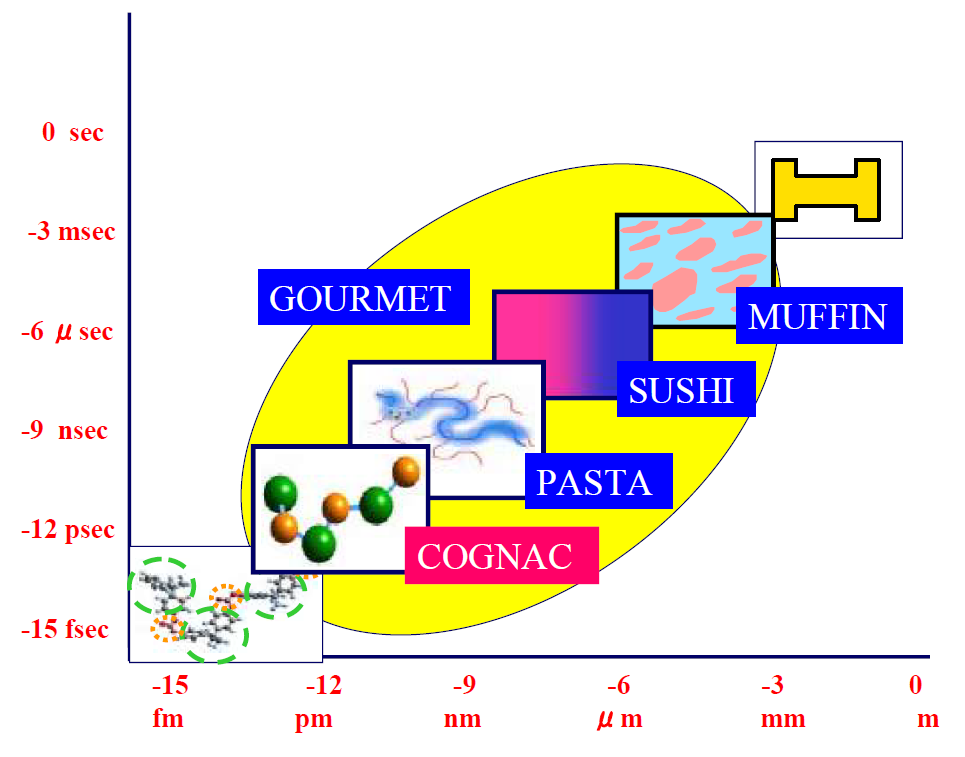
\includegraphics[width=.8\textwidth]{octa.png}
\end{frame}

\begin{frame}
    \frametitle{マルチスケール?}

    \begin{itemize}
        \item マルチスケールが重要なのではなくて、階層的な構造
        \begin{itemize}
            \item 再帰的に捉えることもできるが、
            \begin{itemize}
                \item ローカルには、エントロピー最大化(自由エネルギー最小化)
                \item ローカルの微視的状態の個数倍 $\neq$ グローバル
            \end{itemize}
            \item 準安定状態
            \begin{itemize}
                \item 生物学での、ホメオスタシス(恒常性)
                \item 自己組織化
                \item 分散システムでの自己安定化:フォールトトレラント
            \end{itemize}
        \end{itemize}
        \item マルチフィジックスは、人間の勝手な都合
        \begin{itemize}
            \item 自然はあるがままに捉えるべき
            \item シームレスズーミングは幻想
        \end{itemize}
    \end{itemize}
\end{frame}


\begin{frame}
    \frametitle{自己組織化という概念}
    \begin{block}{自己組織化という概念}
        \begin{itemize}
            \item 材料開発でのナノテクノロジーという文脈で注目
            \item ボトムアップ式のナノテクノロジー
            \item 工学的には、自己集合体とは区別しない事が多い
        \end{itemize}
    \end{block}

    \begin{exampleblock}{自己集合体(平衡条件近傍で形成)とは区別する立場}
        \begin{columns}[T, onlytextwidth]
            \column{.48\linewidth}
            \begin{alertblock}{プリゴジンの散逸構造}
                \begin{itemize}
                    \item 非平衡開放系において
                    \item 平衡構造の不安定化
                    \item 自発的に形成された\\秩序構造
                \end{itemize}
            \end{alertblock}
            \column{.48\linewidth}
            \begin{alertblock}{J.M. Lehn の主張}
                \begin{itemize}
                    \item 超分子科学の提唱者
                    \item 分子自身の分子情報に従って、機能を有する組織を形成
                    % \item 情報の有無に注目
                \end{itemize}
            \end{alertblock}
        \end{columns}
    \end{exampleblock}
\end{frame}

\section{考えてきたこと}
\subsection{化学のやり方}
\begin{frame}
    \frametitle{化学のやり方}
    \begin{itemize}
        \item 基本的には天下りを受容
        \item 見えないものを受け入れる
        \item 
    \end{itemize}
\end{frame}
    
\subsection{物理のやり方}
\begin{frame}
    \frametitle{物理的な考え方}

\end{frame}

\subsection{抽象的?}
\begin{frame}
    \frametitle{抽象}

    「抽象」という語については、「事物や表象からある性質・共通性・本質を抽(ひ)き出して把握する」つまり「象を抽き出す」という意味を持つ語


    \begin{itemize}
        \item 個々の事物の本質・共通の属性を抜き出して、一般的な概念をとらえるさま。
        \item 単に概念的に思考されるだけで、実際の形態・内容を持たないさま。
    \end{itemize}

    後者の意味の反意語は、具体的

    Concrete, Specific

\end{frame}

\begin{frame}
    \frametitle{抽象と捨象}
    \begin{itemize}
        \item 抽き出す行為と捨てる行為
        \item 不要なものに埋もれた中から本質につながる単純化
        \item 粗視化はどちら?
        \item 熊井先生の走り回り画法
    \end{itemize}
\end{frame}


\begin{frame}
    \frametitle{<title>}

    具体的

    Concrete, Specific


    反意語として使われる

    ab-
    struct


\end{frame}
\section{おすすめ}

\subsection{私のやり方}
\begin{frame}
    \frametitle{私のやり方}
        \begin{itemize}
            \LARGE
            \item 急がば回れ
            \begin{itemize}
                \Large
                \item<2-> 慌ててやっても無駄
                \item<2-> キチンと組み立てないと無駄
            \end{itemize}
            \item 備えよ常に
            \begin{itemize}
                \Large
                \item<3-> 見えないものにも前もって
                \item<3-> 泥縄にならないように
            \end{itemize}
            \item 腑に落とす(落ちる)
            \begin{itemize}
                \Large
                \item<4> 消化して使いこなす
                \item<4> 頭でっかちにならない
            \end{itemize}
        \end{itemize}
\end{frame}

\begin{frame}
    \frametitle{基礎知識の汎用化}
        \begin{exampleblock}{データサイエンスの企業での使いこなし}
            \begin{itemize}
                \item データサイエンティストの中途採用
                \begin{itemize}
                    \item マネージメントの難しさ $\Rightarrow$ プロの持ち腐れ
                    \item 現役データサイエンティストの満足度は低い
                    \begin{itemize}
                        \item 手本がない
                        \item 周りの理解がない
                        \item スキルアップの時間がない
                    \end{itemize}
                \end{itemize}
            \end{itemize}
        \end{exampleblock}
        \begin{alertblock}{「データサイエンスの民主化」}
            \begin{itemize}
                \item 文系、数学苦手は関係ない
                \item データをもとに客観的に考えるという基本的な概念
                \item 関係者みんなに広く浅く
                \item 研究一般についても大事
            \end{itemize}
        \end{alertblock}
\end{frame}


\begin{frame}
    \frametitle{概念の理解}
        説明変数と目的変数との関係をモデル化
        \begin{itemize}
            \item 例えば、ランダムフォレスト
            \begin{itemize}
                \item 説明変数の選択への制約が少ない。
                \item 過学習を影響を排除しやすい。
            \end{itemize}
            \item 
            
        \end{itemize}

\end{frame}

\subsection{自分の頭で}
\begin{frame}
    \frametitle{他人の意見について}
        \begin{columns}[c, onlytextwidth]
            \column{.55\linewidth}
            \large
            \begin{block}{その道のプロの言うこと}
                \begin{itemize}
                    \large
                    \item それなりの確からしさ
                    \item 前提条件の確認が必要
                    \item 常識が異なる
                    \item 暗黙の了解が多数
                    \item 素人が下手に使う怖さ
                \end{itemize}
            \end{block}
            \column<2>{.06\linewidth}
            \LARGE
            $\Rightarrow$
            \column<2>{.35\linewidth}
            \Large
                \alert{「盲目的に\\信じてはだめ」}
        \end{columns}
        
        
\end{frame}

\begin{frame}
    \frametitle{自分の頭で考える}
        \begin{alertblock}{胃の腑に落とすということは?}
            無理やり胃に落としてもだめ!!

            \begin{columns}[T, onlytextwidth]
                \column{.48\linewidth}
                
                \begin{block}{咀嚼するための基礎学力}
                    STEAM 
                    \begin{itemize}
                        \item Science
                        \item Technology
                        \item Engineering
                        \item \alert{Art}
                        \begin{itemize}
                            % \item<2> 体系立てて捉える
                            \item<2-> 成り立ちの美しさ
                            \item<2-> 哲学的な統一性 
                        \end{itemize}
                        \item Mathematics
                    \end{itemize}
                \end{block}
                \column{.48\linewidth}
                \begin{exampleblock}<3>{消化(使いこなす)ために?}
                    \begin{itemize}
                        \item 特定の分野に囚われない広範な知見
                        \item 自由な議論
                        \item 締め切りを決めない
                        \item ゆっくり考える
                        \item 数値化にこだわらない
                        \item 目に見えないものを大事に
                    \end{itemize}
                \end{exampleblock}
            \end{columns}
        \end{alertblock}
        
\end{frame}

\end{document}
